\documentclass[../DoAn.tex]{subfiles}
\begin{document}
\section{Khảo sát hiện trạng}
\label{section:2.1}
Hiện nay phần lớn các sàn đấu giá trực tuyến ở Việt Nam thì chủ yếu tập trung vào một nhóm khách hàng hoặc nhóm sản phẩm chủ yếu. Còn sàn đấu giá trực tuyến ở nước ngoài thì không được sử dụng phổ biến tại Việt Nam vì một số vấn đề như quá xa, vận chuyển mất thời gian….

Dưới đây đồ án sẽ trình bày những ưu, nhược điểm của một số sàn đấu giá trực tuyến phổ biến hiện nay ở cả Việt Nam và trên thế giới.

%\begin{table}[]
    %\centering
    \begin{longtable}{| p{.20\textwidth} | p{.25\textwidth} | p{.45\textwidth} |} 
        \caption{Khảo sát và đánh giá các sàn đấu giá trực tuyến hiện nay}
        \label{bang21}
        \endfirsthead
        \endhead
        \hline
        \bfseries Sàn đấu giá & \bfseries Ưu điểm &  \bfseries Nhược điểm\\\hline
        \href{https://www.ebay.com/}{ebay.com} &  ebay.com có sản phẩm đa dạng, phổ biến trên nhiều quốc gia, giao diện thân thiện với người dùng.
        &  ebay.com không được phổ biến ở Việt Nam; không có chuyển đổi thành tiếng Việt; không tìm kiếm phiên đấu giá theo thời gian; không cho phép nhắn tin với người dùng khác.\\\hline
        \href{https://sohot.vn/}{sohot.vn} &  sohot.vn liên kết với website \href{https://www.5giay.vn/}{5giay.vn}, phù hợp với người dùng Việt Nam có nhu cầu về nội thất gia đình.&  sohot.vn có giao diện không thân thiện, khó sử dụng; website chủ yếu bán sản phẩm nội thất gia đình; khi đăng ký phải thông qua 5giay.vn; chỉ tìm kiếm theo tên sản phẩm; không cho phép nhắn tin với người dùng khác.\\\hline
        \href{https://lacvietauction.vn/}{lacvietauction.vn} & lacvietauction.vn có giao diện dễ sử dụng; đảm bảo các tài khoản đăng ký mua bán là chính chủ nên việc xác minh tài khoản thực hiện rất chặt chẽ. & lacvietauction.com chỉ mua bán, đấu giá các sản phẩm có giá trị tương đối lớn như nhà đất, xe ô tô cũ…; chỉ tìm kiếm theo tên của từng nhóm sản phẩm; không cho phép nhắn tin với các người dùng khác .\\\hline
    \end{longtable}
% \end{table}

Về tổng thể các sàn đấu giá này giới hạn nhóm người dùng, nhóm sản phẩm mua bán; bỏ qua tìm kiếm phiên đấu giá theo thời gian; không cho phép nhắn tin với người dùng khác; hoặc sàn đấu giá nước ngoài thì không phù hợp với người Việt Nam. Chính vì những nhược điểm này, website đấu giá trực tuyến mà đồ án xây dựng sẽ cố gắng khắc phục những nhược điểm nói trên, bổ sung thêm các chứng năng khác nhằm phục vụ tốt hơn nhu cầu của người Việt Nam và một bộ phận người Nhật Bản ở Việt Nam.

Website sẽ bao gồm ba đối tượng chính là quản trị viên, người bán và người mua. Quản trị viên có nhiệm vụ quản lý hệ thống bao gồm việc phê duyệt phiên đấu giá; quản lý người dùng; thêm, sửa, xóa loại sản phẩm, thương hiệu, tin tức, slide của website. Người bán sẽ tạo phiên đấu giá về sản phẩm muốn bán. Trong trường hợp người bán có thắc mắc về quá trình tạo phiên đấu giá thì có thể liên lạc với Admin hoặc đọc hướng dẫn tạo phiên đấu giá ở mục tin tức trên Website. Còn người mua thì có thể tham gia các phiên đấu giá đang diễn ra, trả giá cho sản phẩm đó. Khi phiên đấu giá kết thúc, người mua nào đưa ra mức giá cao nhất sẽ được người bán chấp nhận giá và thực hiện giao hàng. Khi người mua nhận được hàng, thực hiện xác nhận và đánh giá sản phẩm, khi đó phiên đấu giá cập nhật trạng thái giao hàng thành công, kết thúc vòng đấu giá.

Mục đích cuối cùng của đồ án là tạo ra một Website có đầy đủ các chức năng cần thiết của một sàn đấu giá trực tuyến và giải quyết các vấn đề còn thiếu của các sàn đấu giá nêu trên.
\section{Tổng quan chức năng}
\label{section:2.2}
\subsection{Biểu đồ use case tổng quát}
\label{subsection:2.2.1}
\begin{figure}[H]
    \centering
    \includegraphics[width=11.4cm,height=13.1cm]{Hinhve/uc tổng quan.png}
    \caption{Biểu đồ usecase Tổng quan}
    \label{fig:Fig21}
\end{figure}
Website đấu giá trên gồm 3 tác nhân chính:

Khách: Là người dùng chưa có tài khoản, người dùng này có thể (i) xem, đọc tin tức; (ii) liên lạc với Admin qua email; (iii) xem thông tin phiên đấu giá trên hệ thống nhưng không thể bình luận hay trả giá. Để có thể sử dụng các chức năng của website thì khách phải tạo tài khoản và đăng nhập.

Người dùng: Là người đã có tài khoản. Người dùng này đăng nhập để sử dụng các chức năng của website như (i) tạo phiên đấu giá, (ii) tham gia đấu giá, (iii) bình luận, (iv) yêu thích, (v) đánh giá sản phẩm, (vi) nhắn tin với người dùng khác, (vii) tìm kiếm phiên đấu giá; (viii) quản lý phiên đấu giá của mình tổ chức như chỉnh sửa, xóa phiên đấu giá chưa được duyệt, chấp nhận giá của người trả giá cao nhất khi phiên đấu giá kết thúc, xác nhận đã giao hàng.

Quản trị viên: Là người quản lý phiên đấu giá, người dùng, loại sản phẩm, thương hiệu, tin tức, slide của toàn bộ website. 
\subsection{Biểu đồ use case phân rã Quản lý người dùng}
\begin{figure}[H]
    \centering
    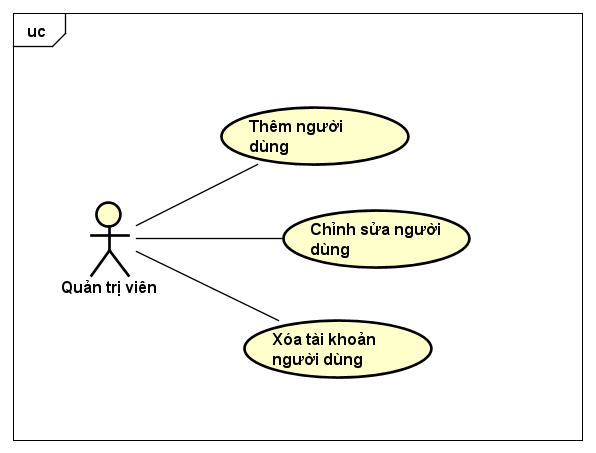
\includegraphics[width=11.4cm,height=8.67cm]{Hinhve/uc quản lý người dùng.png}
    \caption{Biểu đồ usecase Quản lý người dùng}
    \label{fig:Fig22}
\end{figure}
Hình \ref{fig:Fig22} mô tả chức năng Quản lý người dùng. Quản trị viên có thể thêm, chỉnh sửa những tài khoản do Admin tạo, xóa tài khoản không còn hoạt động nữa.
\subsection{Biểu đồ use case phân rã Quản lý phiên đấu giá}
\begin{figure}[H]
    \centering
    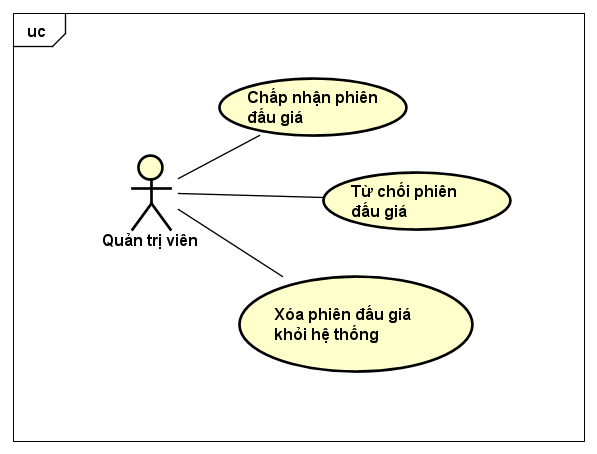
\includegraphics[width=11.4cm,height=8.67cm]{Hinhve/uc quản lý phiên đấu giá.png}
    \caption{Biểu đồ usecase Quản lý phiên đấu giá}
    \label{fig:Fig23}
\end{figure}
Hình \ref{fig:Fig23} mô tả chức năng Quản lý phiên đấu giá. Với chức năng này thì sau khi Người dùng tạo phiên đấu giá, phía Quản trị viên sẽ đánh giá phiên đấu giá đó đủ tiêu chuẩn để duyệt hay chưa. Nếu phiên đấu giá có thông tin không đầy đủ, chính xác thì Quản trị viên có quyền từ chối phiên đấu giá đó và hệ thống sẽ gửi thông báo cho Người tạo phiên đấu giá. Nếu phiên đấu giá được quản trị viên chấp nhận thì hệ thống sẽ cập nhật trạng thái và hiển thị công khai trên website. Với những phiên đấu giá đã được xác nhận giao hàng thành công thì Quản trị viên có thể xóa khỏi hệ thống.
\subsection{Biểu đồ use case phân rã Tạo phiên đấu giá}
\label{subsection:2.2.3}
\begin{figure}[H]
    \centering
    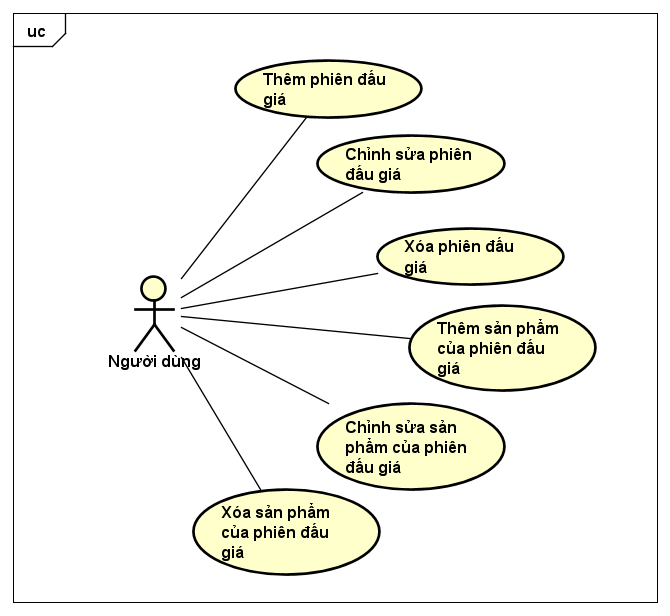
\includegraphics[width=11.4cm,height=10.49cm]{Hinhve/uc tạo phiên đấu giá.png}
    \caption{Biểu đồ usecase Tạo phiên đấu giá}
    \label{fig:Fig24}
\end{figure}
Hình \ref{fig:Fig24} mô tả chức năng Tạo phiên đấu giá của Người dùng. Người dùng có thể thêm mới một phiên đấu giá và thêm sản phẩm cho phiên đấu giá đó. Với những phiên đấu giá chưa được duyệt thì Người dùng có thể chỉnh sửa, xóa sản phẩm và phiên đấu giá đó.
\subsection{Biểu đồ use case phân rã Tìm kiếm thông tin}
\label{subsection:2.2.4}
\begin{figure}[H]
    \centering
    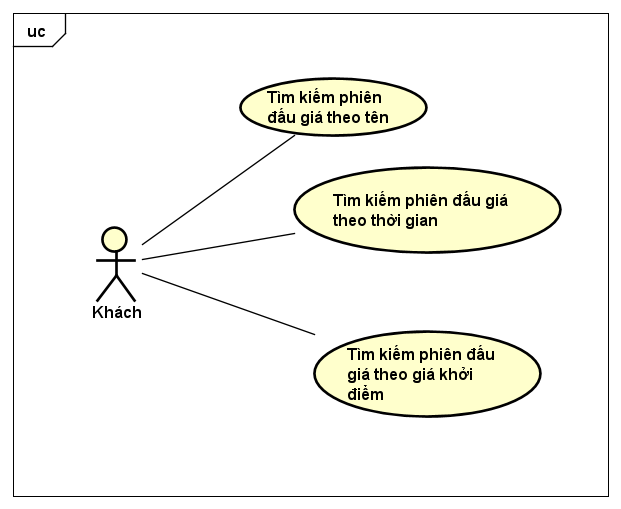
\includegraphics[width=11.4cm,height=9.35cm]{Hinhve/uc tìm kiếm thông tin.png}
    \caption{Biểu đồ usecase Tìm kiếm thông tin}
    \label{fig:Fig25}
\end{figure}
Hình \ref{fig:Fig25} mô tả chức năng Tìm kiếm thông tin. Khách có thể tìm kiếm các phiên đấu giá theo tên, theo thời gian bắt đầu, thời gian kết thúc và theo giá khởi điểm. 
\subsection{Biểu đồ use case phân rã Nhắn tin trực tuyến}
\label{subsection:2.2.6}
\begin{figure}[H]
    \centering
    \includegraphics[width=9.9cm,height=6.11cm]{Hinhve/uc nhắn tin.png}
    \caption{Biểu đồ usecase Nhắn tin trực tuyến}
    \label{fig:Fig26}
\end{figure}
Hình \ref{fig:Fig26} mô tả chức năng Nhắn tin trực tuyến trên hệ thống. Người dùng chọn vào hình nền mà mình muốn nhắn tin để bắt đầu cuộc trò chuyện. Nhập nội dung tin nhắn sau đó ấn gửi để gửi nội dung đến người dùng khác. 
\subsection{Quy trình nghiệp vụ}
\label{subsection:2.2.7}
\subsubsection{Nghiệp vụ tạo phiên đấu giá}
\label{subsubsection:2.2.7.1}
\begin{figure}[H]
    \centering
    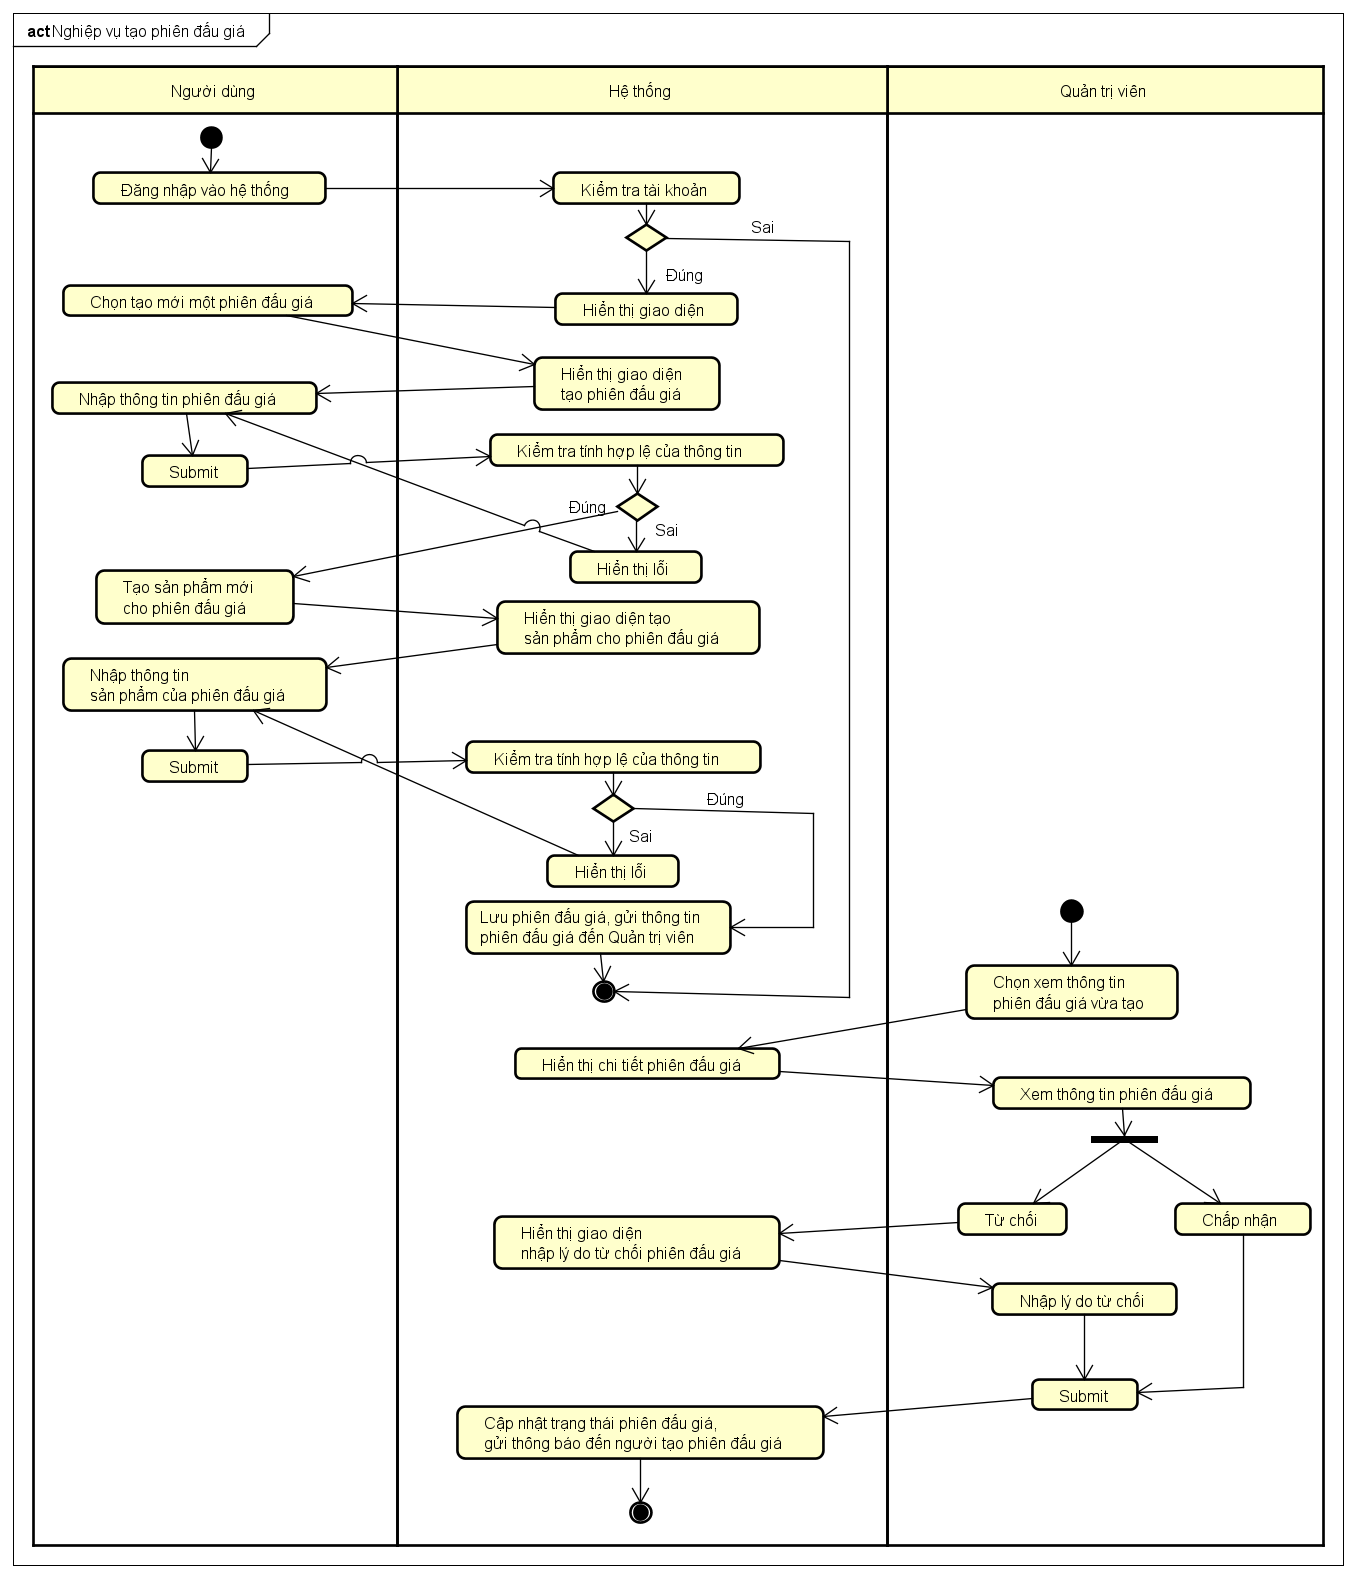
\includegraphics[width=11.4cm,height=13.28cm]{Hinhve/nghiệp vụ tạo phiên đấu giá.png}
    \caption{Nghiệp vụ tạo phiên đấu giá}
    \label{fig:Fig27}
\end{figure}
Hình \ref{fig:Fig27} mô tả nghiệp vụ tạo một phiên đấu giá. Người dùng đăng nhập vào hệ thống, chọn mục Bán hàng để tạo mới một phiên đấu giá. Người dùng nhập các thông tin theo form tạo mới phiên đấu giá, nếu thông tin không hợp lệ thì hệ thống sẽ báo lỗi ngay dưới trường đó. Sau khi tạo phiên đấu giá thành công thì hệ thống sẽ chuyển qua giao diện tạo mới sản phẩm cho phiên đấu giá đó. Tương tự người dùng cần nhập thông tin đầy đủ và hợp lệ, nếu không thì hệ thống sẽ báo lỗi ngay dưới trường không hợp lệ. Sau khi tạo mới sản phẩm xong thì người dùng phải đợi phía Admin phê duyệt. Phía Admin có nhiệm vụ chấp nhận hay từ chối phiên đấu giá, sau đó hệ thống sẽ cập nhật lại trạng thái phiên đấu giá.
\subsubsection{Nghiệp vụ tạo phiên đấu giá}
\label{subsubsection:2.2.7.2}
\begin{figure}[H]
    \centering
    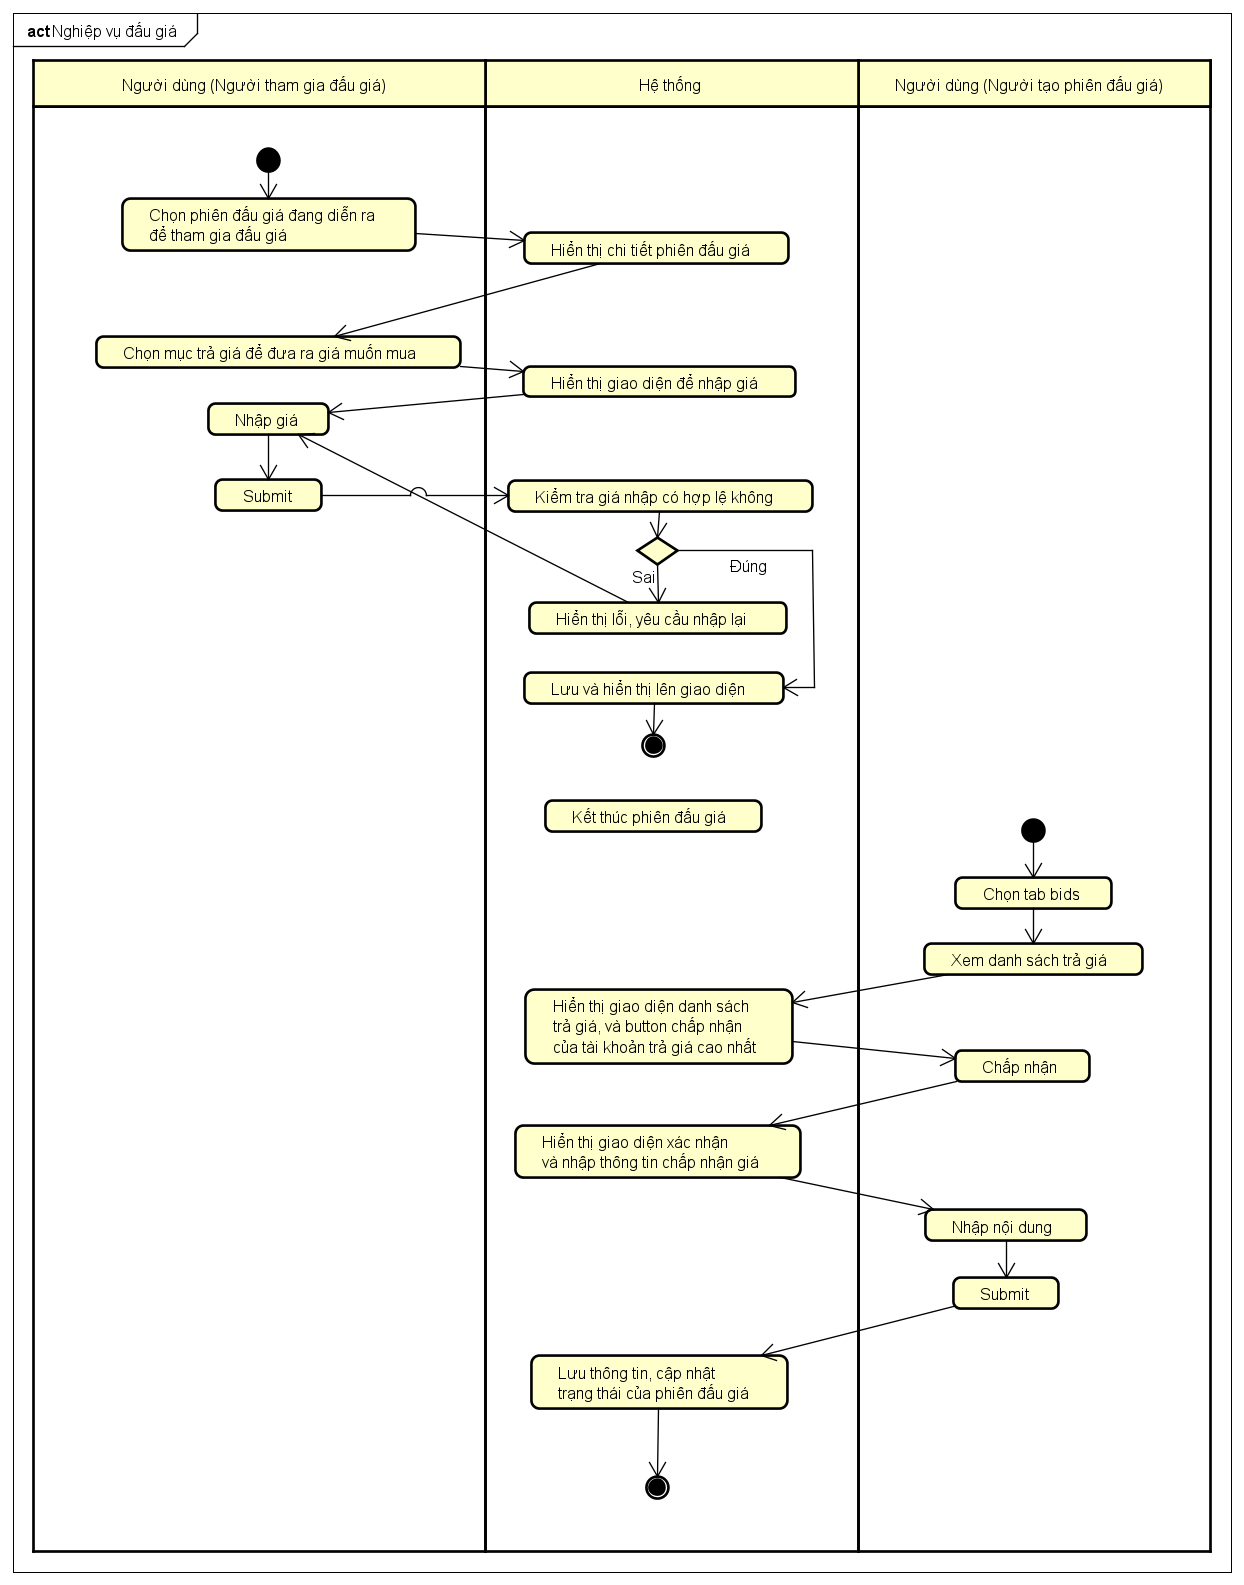
\includegraphics[width=11.4cm,height=14.54cm]{Hinhve/nghiệp vụ đấu giá.png}
    \caption{Nghiệp vụ tạo phiên đấu giá}
    \label{fig:Fig28}
\end{figure}
Hình \ref{fig:Fig28} mô tả nghiệp vụ Đấu giá. Khi một phiên đấu giá đang diễn ra thì Người dùng có thể tham gia trả giá. Người dùng chọn mục trả giá, nhập giá hợp lệ. Nếu giá mà người dùng đưa ra không lớn hơn trả giá cao nhất hiện tại hay không phải là số thì hệ thống sẽ báo lỗi dưới ô nhập giá. Khi phiên đấu giá kết thúc thì tại tài khoản của Người tạo phiên đấu giá đó sẽ hiển thị nút Chấp nhận với lượt trả giá cao nhất. Sau khi Người tạo phiên đấu giá xác nhận thì Hệ thống cập nhật trạng thái phiên đấu giá.
\section{Đặc tả chức năng}
\label{section:2.3}
\subsection{Đặc tả use case Tạo phiên đấu giá}
%\begin{table}[H]
    %\centering
    \begin{longtable}{| p{.25\textwidth} | p{.15\textwidth} | p{.15\textwidth} | p{.30\textwidth} |} 
    \caption{Đặc tả usecase Tạo phiên đấu giá}
    \label{bang22}
    \endfirsthead
    \endhead
    \hline
        \bfseries Mã Use case & \bfseries UC0001 & \bfseries Tên Use case & \bfseries Tạo phiên đấu giá \\\hline
        \bfseries Tác nhân hệ thống & \multicolumn{3}{c|}{Người dùng} \\\hline
        \bfseries Tiền điều kiện & \multicolumn{3}{c|}{Đăng nhập} \\\hline
        \bfseries Luồng sự kiện chính & \multicolumn{3}{c|}{
        \begin{tabular}{| p{.05\textwidth} | p{.15\textwidth} | p{.40\textwidth} |} 
            \hline
                \bfseries STT & \bfseries Thực hiện &  \bfseries Hành động \\\hline
                1 & Người dùng & Chọn chức năng tạo mới phiên đấu giá \\\hline
                2 & Hệ thống & Hiển thị giao diện tạo phiên đấu giá \\\hline
                3 & Người dùng & Nhập thông tin phiên đấu giá. Nhấn xác nhận \\\hline
                4 & Hệ thống & Kiểm tra tính hợp lệ của các trường thông tin mà Người dùng đã nhập \\\hline
                5 & Hệ thống & Lưu trữ thông tin phiên đấu giá vào cơ sở dữ liệu. Chuyển hướng qua trang tạo sản phẩm cho phiên đấu giá \\\hline
                6 & Hệ thống & Hiển thị thông tin của phiên đấu giá vừa tạo và giao diện để tạo sản phẩm cho phiên đấu giá \\\hline
                7 & Người dùng & Nhập thông tin sản phẩm cho phiên đấu giá tương ứng và xác nhận \\\hline
                8 & Hệ thống & Kiểm tra tính hợp lệ của các trường thông tin.  \\\hline
                9 & Hệ thống & Lưu thông tin sản phẩm vào cơ sở dữ liệu. Chuyển hướng đến trang cá nhân của người dùng đang đăng nhập \\\hline
        \end{tabular}
        }\\\hline
        \bfseries Luồng sự thay thế & \multicolumn{3}{c|}{
        \begin{tabular}{| p{.05\textwidth} | p{.15\textwidth} | p{.40\textwidth} |} 
            \hline
                \bfseries STT & \bfseries Thực hiện &  \bfseries Hành động \\\hline
                4a & Hệ thống & Thông báo các trường yêu cầu phải nhập, hoặc các giá trị nhập không hợp lệ \\\hline
                8a & Hệ thống & Thông báo các trường yêu cầu phải nhập, hoặc các giá trị nhập không hợp lệ \\\hline
        \end{tabular}
        }\\\hline
        \bfseries Hậu điều kiện & \multicolumn{3}{c|}{Không}\\\hline
    \end{longtable}
%\end{table}
\subsection{Đặc tả use case Từ chối phiên đấu giá}
%\begin{table}[H]
    %\centering
    \begin{longtable}{| p{.25\textwidth} | p{.15\textwidth} | p{.15\textwidth} | p{.30\textwidth} |} 
    \caption{Đặc tả usecase Từ chối phiên đấu giá}
    \label{bang23}
    \endfirsthead
    \endhead
    \hline
        \bfseries Mã Use case & \bfseries UC0002 & \bfseries Tên Use case & \bfseries Từ chối phiên đấu giá \\\hline
        \bfseries Tác nhân hệ thống & \multicolumn{3}{c|}{Quản trị viên} \\\hline
        \bfseries Tiền điều kiện & \multicolumn{3}{c|}{Đăng nhập với vai trò là quản trị viên} \\\hline
        \bfseries Luồng sự kiện chính & \multicolumn{3}{c|}{
        \begin{tabular}{| p{.05\textwidth} | p{.15\textwidth} | p{.40\textwidth} |} 
            \hline
                \bfseries STT & \bfseries Thực hiện &  \bfseries Hành động \\\hline
                1 & Quản trị viên & Chọn danh sách phiên đấu giá đang chờ duyệt \\\hline
                2 & Quản trị viên & Chọn vào phiên đấu giá muốn phê duyệt \\\hline
                3 & Hệ thống & Hiển thị thông tin chi tiết của phiên đấu giá đó \\\hline
                4 & Quản trị viên & Chọn từ chối \\\hline
                5 & Hệ thống & Lưu trữ thông tin phiên đấu giá vào cơ sở dữ liệu. Chuyển hướng qua trang tạo sản phẩm cho phiên đấu giá \\\hline
                6 & Quản trị viên & Nhập lý do từ chối, xác nhận \\\hline
                7 & Hệ thống & Kiểm tra tính hợp lệ của thông tin\\\hline
                8 & Hệ thống & Lưu lý do từ chối phiên đấu giá và gửi thông báo đến Người dùng. Cập nhật trạng thái của phiên đấu giá  \\\hline
                9 & Hệ thống & Chuyển hướng về danh sách phiên đấu giá chờ duyệt \\\hline
        \end{tabular}
        }\\\hline
        \bfseries Luồng sự thay thế & \multicolumn{3}{c|}{
        \begin{tabular}{| p{.05\textwidth} | p{.15\textwidth} | p{.40\textwidth} |} 
            \hline
                \bfseries STT & \bfseries Thực hiện &  \bfseries Hành động \\\hline
                7a & Hệ thống & Thông báo cần nhập lý do từ chối nếu Quản trị viên không nhập lý do mà xác nhận luôn. \\\hline
        \end{tabular}
        }\\\hline
        \bfseries Hậu điều kiện & \multicolumn{3}{c|}{Không}\\\hline
    \end{longtable}
%\end{table}
\subsection{Đặc tả use case Chấp nhận giá}
%\begin{table}[H]
    %\centering
    \begin{longtable}{| p{.25\textwidth} | p{.15\textwidth} | p{.15\textwidth} | p{.30\textwidth} |} 
    \caption{Đặc tả usecase Chấp nhận giá}
    \label{bang24}
    \endfirsthead
    \endhead
    \hline
        \bfseries Mã Use case & \bfseries UC0003 & \bfseries Tên Use case & \bfseries Chấp nhận giá \\\hline
        \bfseries Tác nhân hệ thống & \multicolumn{3}{c|}{Người dùng} \\\hline
        \bfseries Tiền điều kiện & \multicolumn{3}{c|}{Đăng nhập} \\\hline
        \bfseries Luồng sự kiện chính & \multicolumn{3}{c|}{
        \begin{tabular}{| p{.05\textwidth} | p{.15\textwidth} | p{.40\textwidth} |} 
            \hline
                \bfseries STT & \bfseries Thực hiện &  \bfseries Hành động \\\hline
                1 & Người dùng & Chọn chấp nhận\\\hline
                2 & Hệ thống & Hiển thị giao diện nhập thông tin thêm về việc chấp nhận giá \\\hline
                3 & Người dùng & Nhập thông tin, Xác nhận\\\hline
                4 & Hệ thống & Kiểm tra tính hợp lệ của thông tin \\\hline
                5 & Hệ thống & Lưu thông tin vào cơ sở dữ liệu, cập nhật trạng thái của phiên đấu giá\\\hline
                6 & Hệ thống & Chuyển hướng đến trang cá nhân của người dùng đang đăng nhập \\\hline
        \end{tabular}
        }\\\hline
        \bfseries Luồng sự thay thế & \multicolumn{3}{c|}{
        \begin{tabular}{| p{.05\textwidth} | p{.15\textwidth} | p{.40\textwidth} |} 
            \hline
                \bfseries STT & \bfseries Thực hiện &  \bfseries Hành động \\\hline
                4a & Hệ thống & Thông báo yêu cầu nhập khi người dùng không nhập thông tin về việc chấp nhận giá mà xác nhận luôn. \\\hline
        \end{tabular}
        }\\\hline
        \bfseries Hậu điều kiện & \multicolumn{3}{c|}{Không}\\\hline
    \end{longtable}
%\end{table}
\subsection{Đặc tả use case Tìm kiếm thông tin}
%\begin{table}[H]
    %\centering
    \begin{longtable}{| p{.25\textwidth} | p{.15\textwidth} | p{.15\textwidth} | p{.30\textwidth} |} 
    \caption{Đặc tả usecase Tìm kiếm thông tin}
    \label{bang25}
    \endfirsthead
    \endhead
    \hline
        \bfseries Mã Use case & \bfseries UC0004 & \bfseries Tên Use case & \bfseries Tìm kiếm thông tin \\\hline
        \bfseries Tác nhân hệ thống & \multicolumn{3}{c|}{Khách} \\\hline
        \bfseries Tiền điều kiện & \multicolumn{3}{c|}{Không} \\\hline
        \bfseries Luồng sự kiện chính & \multicolumn{3}{c|}{
        \begin{tabular}{| p{.05\textwidth} | p{.15\textwidth} | p{.40\textwidth} |} 
            \hline
                \bfseries STT & \bfseries Thực hiện &  \bfseries Hành động \\\hline
                1 & Khách & Chọn loại Tìm kiếm thông tin \\\hline
                2 & Khách & Nhập từ khóa tìm kiếm, nhấn vào icon tìm kiếm \\\hline
                3 & Hệ thống & Tìm kiếm trong hệ thống theo từ khóa và nhóm tìm kiếm mà Khách đã chọn. \\\hline
                4 & Hệ thống & Hiển thị các kết quả tìm kiếm \\\hline
        \end{tabular}
        }\\\hline
        \bfseries Luồng sự thay thế & \multicolumn{3}{c|}{
        \begin{tabular}{| p{.05\textwidth} | p{.15\textwidth} | p{.40\textwidth} |} 
            \hline
                \bfseries STT & \bfseries Thực hiện &  \bfseries Hành động \\\hline
                4a & Hệ thống & Nếu không tìm thấy kết quả nào thì hệ thống không hiển thị thông tin gì.\\\hline
        \end{tabular}
        }\\\hline
        \bfseries Hậu điều kiện & \multicolumn{3}{c|}{Không}\\\hline
    \end{longtable}
%\end{table}
\subsection{Đặc tả use case Đánh giá}
%\begin{table}[H]
    %\centering
    \begin{longtable}{| p{.25\textwidth} | p{.15\textwidth} | p{.15\textwidth} | p{.30\textwidth} |} 
    \caption{Đặc tả usecase Đánh giá}
    \label{bang26}
    \endfirsthead
    \endhead
    \hline
        \bfseries Mã Use case & \bfseries UC0005 & \bfseries Tên Use case & \bfseries Đánh giá \\\hline
        \bfseries Tác nhân hệ thống & \multicolumn{3}{c|}{Đánh giá} \\\hline
        \bfseries Tiền điều kiện & \multicolumn{3}{c|}{Đã đăng nhập, sau khi nhận được hàng} \\\hline
        \bfseries Luồng sự kiện chính & \multicolumn{3}{c|}{
        \begin{tabular}{| p{.05\textwidth} | p{.15\textwidth} | p{.40\textwidth} |} 
            \hline
                \bfseries STT & \bfseries Thực hiện &  \bfseries Hành động \\\hline
                1 & Khách & Chọn Đã nhận được hàng \\\hline
                2 & Hệ thống & Hiển thị form đánh giá sản phẩm của phiên đấu giá \\\hline
                3 & Khách & Nhập các thông tin, xác nhận \\\hline
                4 & Hệ thống & Kiểm tra tính hợp lệ của thông tin \\\hline
                5 & Hệ thống & Lưu thông tin đánh giá vào cơ sở dữ liệu. \\\hline
        \end{tabular}
        }\\\hline
        \bfseries Luồng sự thay thế & \multicolumn{3}{c|}{
        \begin{tabular}{| p{.05\textwidth} | p{.15\textwidth} | p{.40\textwidth} |} 
            \hline
                \bfseries STT & \bfseries Thực hiện &  \bfseries Hành động \\\hline
                4a & Hệ thống & Thông báo lỗi khi người dùng không nhập thông tin các trường cần thiết hay nhập sai định dạng. \\\hline
        \end{tabular}
        }\\\hline
        \bfseries Hậu điều kiện & \multicolumn{3}{c|}{Không}\\\hline
    \end{longtable}
%\end{table}
\section{Yêu cầu phi chức năng}
\label{section:2.4}
\subsection{Yêu cầu về kỹ thuật}
\label{subsection:2.4.1}
\begin{itemize}
    \item Website phân quyền người sử dụng: tùy theo từng nhóm người dùng sẽ có những quyền hạn truy cập, sử dụng những tính năng nhất định. 
    \item Sử dụng Single Page nên thời gian phản hồi giữa các màn hình nằm trong giới hạn cho phép.
    \item Phản hồi các thao tác của người dùng nhanh chóng.
    \item Hệ thống hoạt động ổn định, trong thời gian làm việc không gặp lỗi quá lớn.
    \item Hệ thống đảm bảo tính dễ bảo trì, dễ mở rộng trong tương lai
\end{itemize}
\subsection{Yêu cầu về giao diện}
\label{subsection:2.4.2}
\begin{itemize}
    \item Giao diện đẹp, đơn giản, dễ sử dụng, thân thiện với người dùng
    \item Hệ thống thông báo lỗi rõ ràng, chính xác trong các trường hợp người dùng nhập các trường thông tin không hợp lệ.
    \item Các nút, tiêu đề rõ ràng, dễ hiểu, có tính gợi nhớ
    \item Thực hiện phân trang để chia nhỏ những danh sách quá dài
\end{itemize}

%%%%%%%%%%%%%%%%%%%%%%%%%%%%%%%%%%%

\end{document}